As of the current moment the forecast component diagram for the system is as follows:

\begin{figure}[!htpb]
    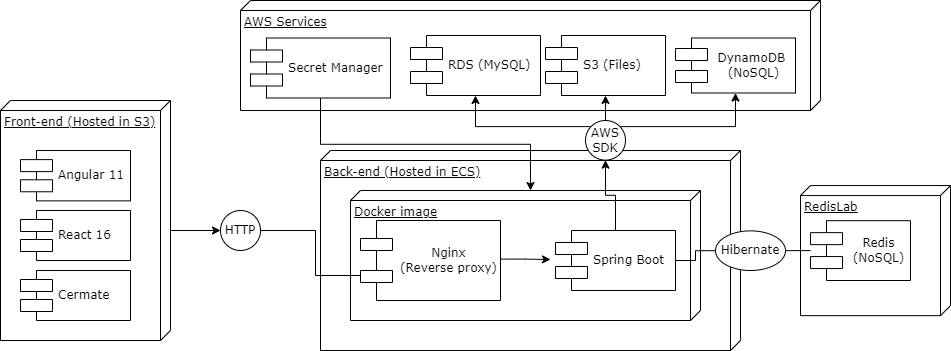
\includegraphics[width=0.9\textwidth]{images/forecast}
    \caption{\footnotesize{Forecast component diagram}}
    \label{fig:forecast}
\end{figure}

As it's shown in \ref{fig:forecast} there are additional databases that are waiting to get
implemented mainly ones for archiving files as is the case of S3 and also archiving data
of the trucks and drivers that could be used for statistics and KPIs down the line thus
using DynamoDB\@.

The containerization of the system to be done in the future as follows,
first the creatoin of a docker image of the system
then the deployment of the image to ECR
and finally turning up ECS task to take care of the management of the system.

An addition of a deployment system such as CI/CD pipelines to be able to
deploy the system seamlessly and in a way that is easy to use and maintain.

Finally, turning back to what's within the code base, is the creation of
new model to be followed within the system and the creation of new
componenets and features that were missing before hand, such as 
a user management system which would allow having the proper access 
to the system and adding some security measures to the backend is a set target
such as the rework of authentication handling, and the rate limiting of the API
to prevent the system from being flooded with requests.

